\section{Event reconstruction and particle identification}
%%%%%%%%%%%%%%%%%%%%%%%%%%%%%%%%%%%%%%%%%%%%%%%%%%%%%%
\label{sec:Objects}

In CMS, the physics object reconstruction and identification is based on standard algorithms developed by the collaboration and used by all the physics analyses. In this section, the techniques used for the reconstruction and identification of the physics objects of interest for \hwwllnn analyses are described.

\subsection{The Particle Flow technique}

The Particle Flow (PF) event reconstruction technique~\cite{CMS-PAS-PFT-09-001} aims at the reconstruction and identification of all the stable particles in the event, i.e. electrons, muons, photons, charged and neutral hadrons, with a thorough combination of the information from all CMS sub-detectors, in order to determine their energy, direction and type. These individual particles are then used, for example, to build jets, to measure the missing transverse energy \MET, to reconstruct the $\tau$ from their decay products, to quantify the charged lepton isolation and to tag b-jets.

The CMS detector is well suited for this purpose. Indeed, the presence of a large internal silicon tracker immersed in an intense solenoidal magnetic field allows the reconstruction of charged particles with high efficiency and small fake rate, and provides a high precision measurement of the particle \pt down to about $150\,\MeV$, for $|\eta|\leq2.6$. The high granularity of the ECAL calorimeter is the additional key element for the feasibility of the PF technique, allowing the reconstruction of photons and electrons with high energy resolution.

The first step of the PF technique consists in the reconstruction of the basic elements from the various sub-detectors, such as charged-particle tracks, calorimeter clusters and muon tracks. These elements, which are provided by the sub-detectors with high efficiency an low fake rate, are then connected together with a link algorithm.

The good performance of the tracking system are achieved by means of an iterative tracking strategy~\cite{Chatrchyan:2014fea}, based on the Kalman Filter algorithm~\cite{Billoir:1990we}. The basic idea of iterative tracking is that initial iterations search for tracks that are easiest to find, e.g. high \pt tracks produced near the interaction region. After each iteration, hits associated to reconstructed tracks are removed from the hit collection, thereby reducing the combinatorial complexity and simplifying the subsequent iterations, which aim at finding more complicated set of tracks, e.g. low \pt or displaced tracks. The \emph{Iteration 0}, where the majority of tracks are reconstructed, is designed to identify prompt tracks with $\pt>0.8$\,\GeV that have three hits in the three layers of the pixel detector. \emph{Iteration 1} is used to recover prompt tracks that have only two pixel hits. \emph{Iteration 2} aims at finding low-\pt prompt tracks while \emph{Iterations 3--5} are intended to find tracks that originate outside the collision point, i.e. tracks produced by a secondary vertex, and to recover undetected tracks in the previous iterations. Each iteration proceeds according to four steps:
\begin{itemize}
\item \emph{seeding}: initial track candidates are obtained using 2 or 3 hits in the innermost layers (these proto-tracks are called seeds);
\item \emph{pattern recognition}: this step is based on Kalman Filter and searches for hits in the outer layers that could be associated to the initial track candidate, reconstructing the particle trajectory;
\item \emph{track fitting}: in this step a fit of the trajectory is performed, using its associated hits and providing an estimate of the track parameters (\pt, $\eta$, $\phi$, charge, etc.);
\item \emph{selection}: finally tracks are selected based on quality requirements.
\end{itemize}

The high detection efficiency of the calorimeters is based on a specific calorimeter clustering algorithm, which is performed separately in each sub-detector. The algorithm is based on three steps: in the first step, ``cluster seeds'' are identified as local calorimeter cells with an energy deposit above a given threshold. Then, ``topological clusters'' are grown from the seeds by gathering cells with at least one side in common with a cell already in the cluster, and with an energy above a given threshold. A topological cluster usually gives rise to many ``particle flow clusters'' as seeds, which are identified sharing the energy of each cell among the particle flow clusters, thereby allowing the determination of the particle flow cluster energy and position.

These elements are then connected to each other using a link algorithm, which identifies blocks of elements that are topologically compatible. For example, a charged-particle track is linked to a calorimeter particle flow cluster if the extrapolated position from the track to the calorimeter is compatible with the cluster boundaries. From these blocks, PF candidates are identified according to the following order:
\begin{itemize}
\item Muons: a \emph{global muon} gives rise to a \emph{PF muon} if its combined \pt measurement is compatible within 3 standard deviation with the one provided by the sole tracker. The corresponding track is removed from the block;
\item Electrons: electrons tend to give rise to short tracks, and to lose energy by Bremsstrahlung in the tracker layers on their way to the calorimeter. The link between a charged-particle track (refitted with the Gaussian-Sum Filter (GSF)~\cite{Adam:815410}) and one or more ECAL clusters identifies a \emph{PF electron}. After the identification, the corresponding tracks and clusters are removed from the block.
\item Charged hadrons: the remaining tracks give rise to \emph{PF charged hadrons}. Tracks can be linked to ECAL and HCAL clusters, and the energy is determined taking into account information from calorimeters;
\item Photons and neutral hadrons: ECAL clusters not linked with tracks give rise to \emph{PF photons}, while the remaining HCAL clusters are identified as \emph{PF neutral hadrons}.
\end{itemize}
After the identification of all PF candidates in the event, \emph{PF jets} are clustered as described in Sec.~\ref{chap2:jets}. The last step is the reconstruction of the \emph{PF \ptmiss}, which is given by:

\begin{equation} 
\ptmiss = - \sum_{\mathrm{PF\,obj}} \vec{p}_\mathrm{T}^\mathrm{\,PF\,obj} \quad,
\end{equation}

where the sum extends over all the PF objects. The \MET is defined as the modulus of \ptmiss.

\subsection{Leptons reconstruction and identification}

\subsubsection{Muon reconstruction and identification}
Muons produced at the collision point can go through the entire detector with a negligible energy loss, thus reaching the detector outermost part where the muon chambers are installed (see Sec.~\ref{sec:muonsyst}). Muons interact through ionization with the layers of the silicon tracker, which is able to reconstruct their tracks (\emph{tracker track}). The muon tracks are also reconstructed using the muon system (\emph{standalone muon track}). Based on these objects, two reconstruction approaches are used~\cite{Chatrchyan:2012xi}: in the first method (outside-in), for each standalone muon tracks a tracker track is searched for by extrapolating the two tracks to a common surface. If a match is found, the hits associated to the two tracks are fitted together giving rise to a \emph{Global Muon}. The second approach (inside-out) consists in considering all tracker tracks with $\pt > 0.5$\,\GeV as potential muon candidates and are extrapolated to the muon system taking into account the magnetic field, the expected energy losses and the multiple scattering in the detector material. If at least one muon segment (a short track stub made of DT or CSC hits) matches the extrapolated tracks, the corresponding tracker track is identified as a \emph{Tracker Muon}.

The matching with the muon system improves significantly the muon \pt resolution that can be obtained from the tracker only, especially in the region with $\pt > 200$\GeV, as shown in Fig.~\ref{fig:muptres}. 
\begin{figure}[htb]
\centering
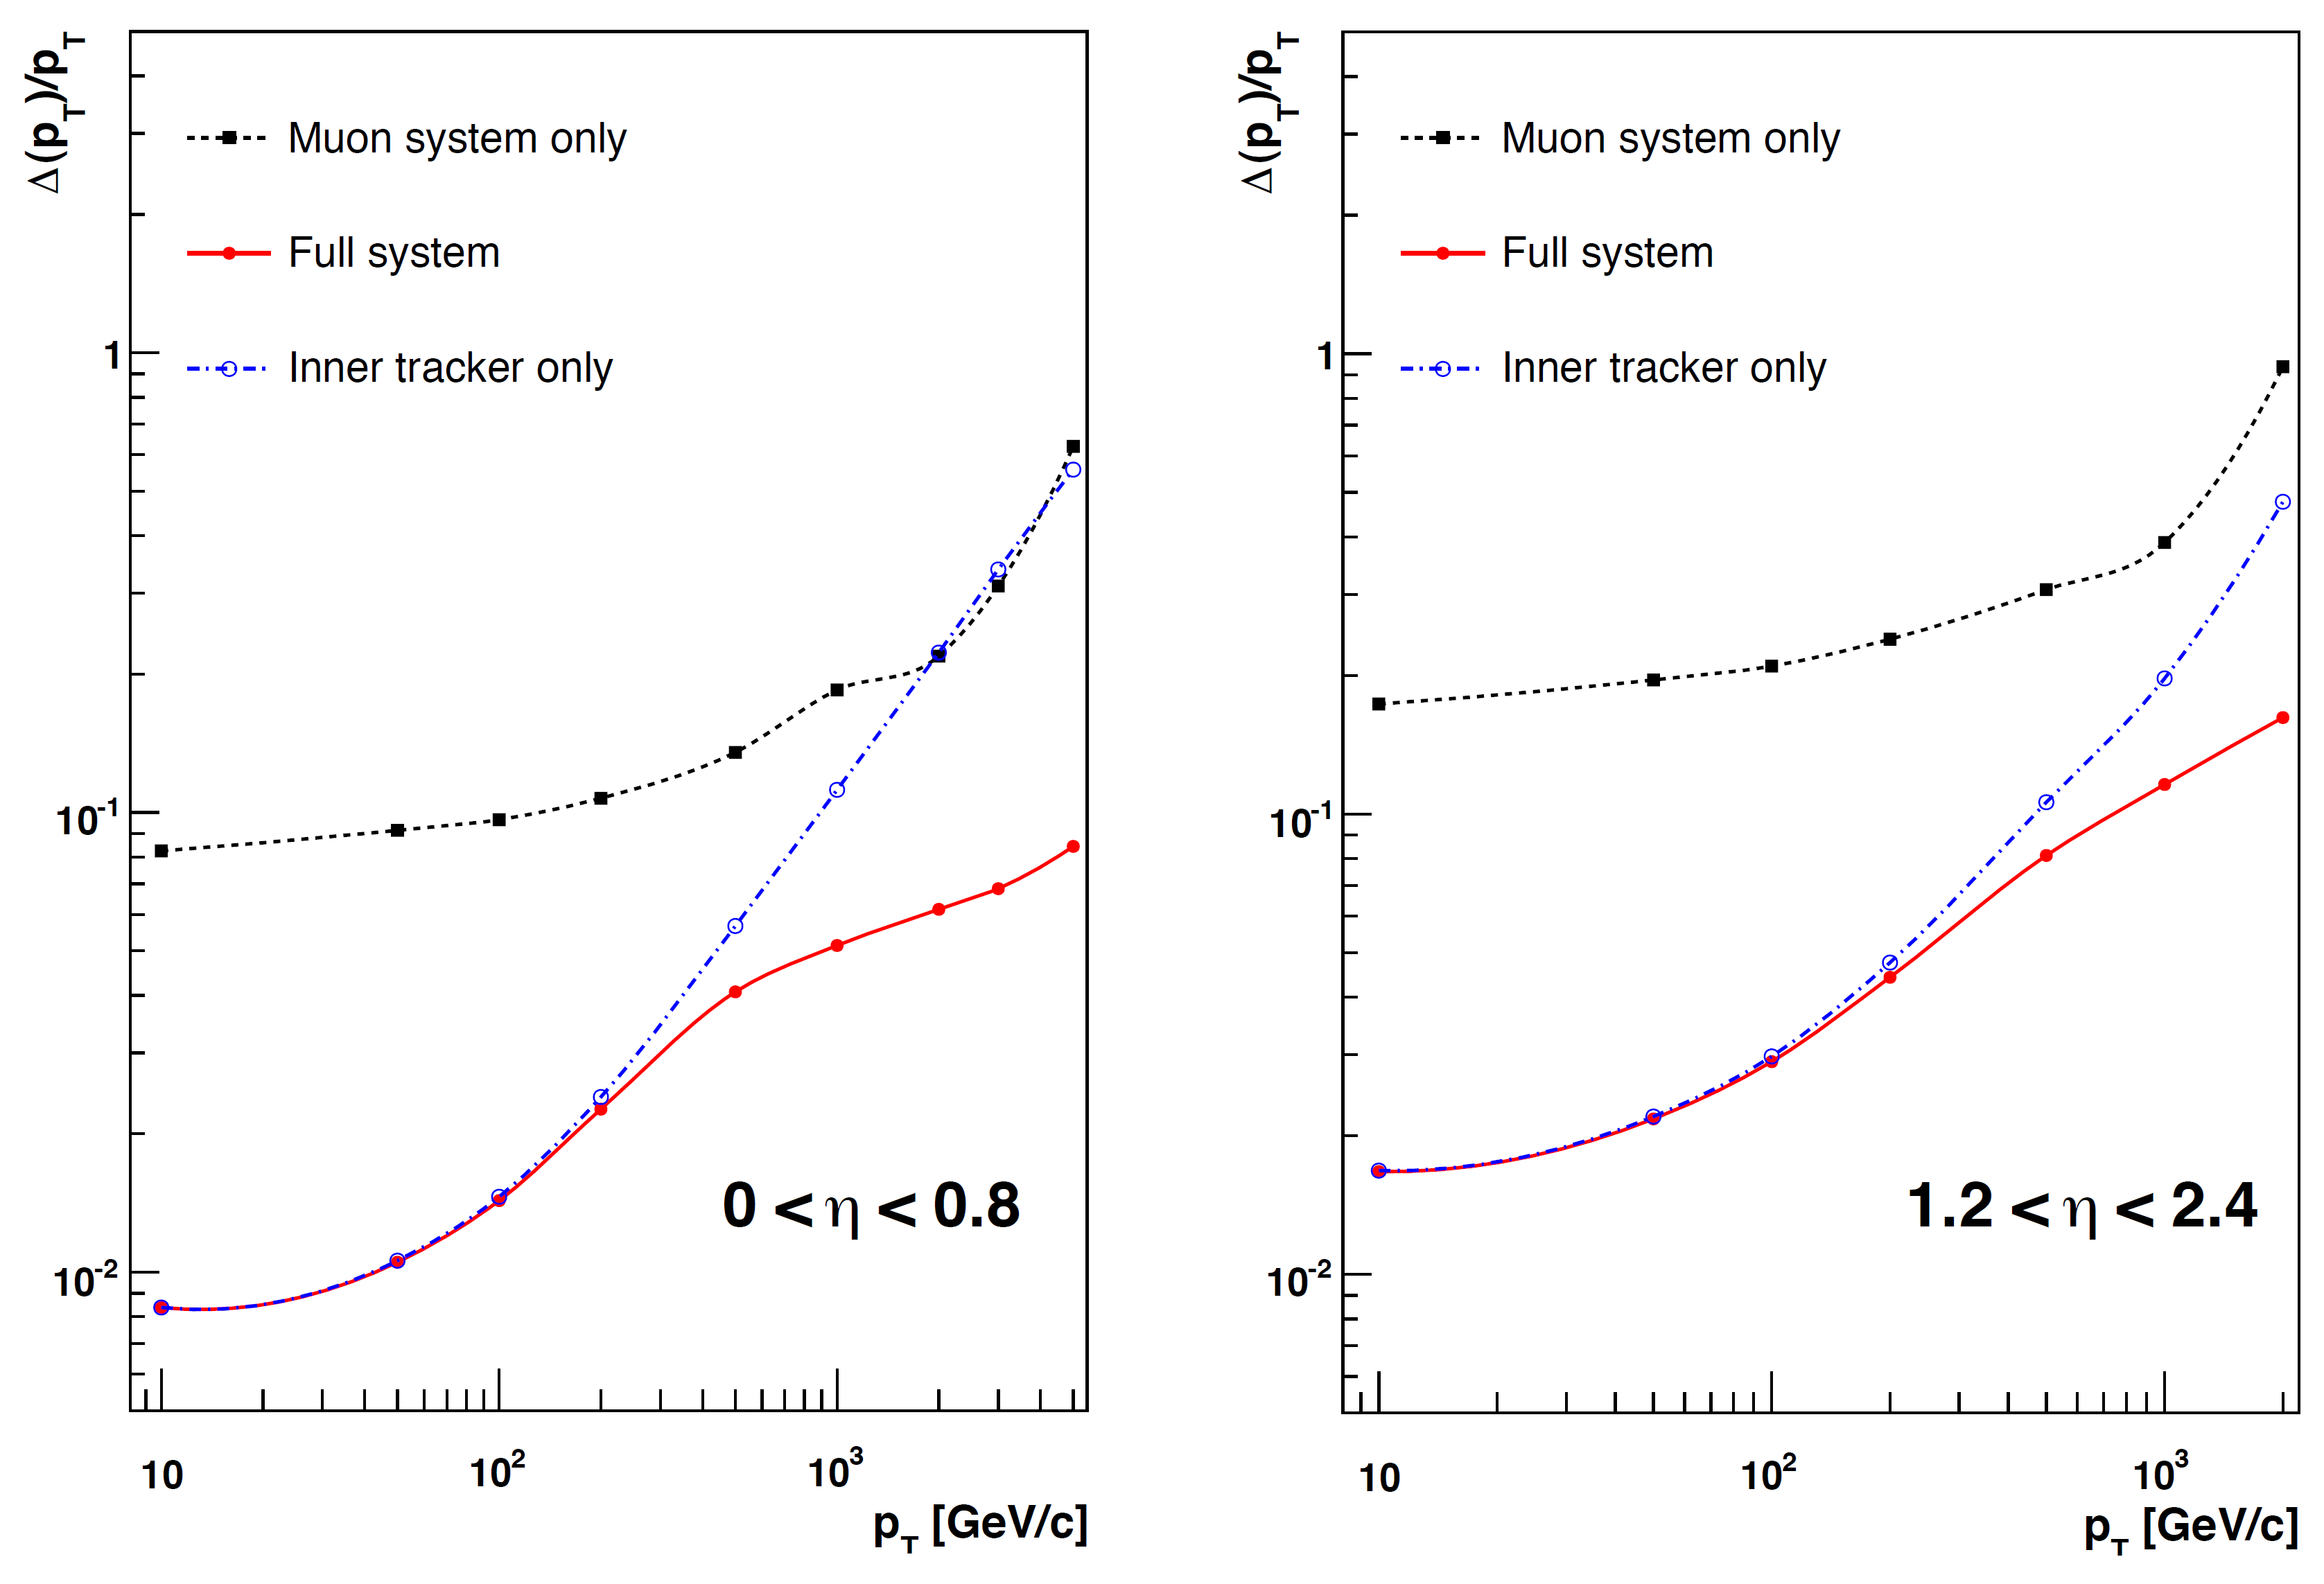
\includegraphics[width=0.6\textwidth]{images/muptres.png}
\caption{Muon \pt resolution as a function of the muon \pt in the barrel (left) and in the endcap (right) regions. The resolution is provided for the measurement using the tracking system or the muon system only, as well as for the combination of the two methods.}\label{fig:muptrese}
\end{figure}

Depending on the physics analysis, different muon definitions can be used by changing the selection on the muon identification variables, hence balancing between the muon identification efficiency and purity. The most widely used definition in physics analyses is the so-called \emph{Tight muon selection}\footnote{Small variations with respect to this baseline definition are adopted by the specific analyses.}. This selection requires the muon candidate to be reconstructed as a Global Muon and identified by the PF algorithm. The fit of the global track, which is required to include muon segments in at least two muon stations (this implies that the muon is also reconstructed as a Tracker Muon), must have a $\chi^2/d.o.f.$ less than 10 and use more than 10 inner tracker hits. The transverse impact parameter with respect to the primary vertex is required to be $|d_{xy}|<2$\,mm, significantly reducing the rate of muons from decays in flight, i.e. non prompt muons. The requirements defining the Tight Muon identification are summarized in Table~\ref{tab:tightmuon}.

\begin{table}[htb]
\caption{Summary of the muon identification variables and the corresponding selections commonly used by physics analyses.}\label{tab:tightmuon}
\centering
\begin{tabular}{lc}
\toprule \\
Observable & Cut \\
\midrule \\
Is Global Muon & true \\
Is PF muon & true \\
Tracker layers with valid hits & $>5$ \\
Number of valid pixel hits & $>0$ \\
Number of valid muon hits & $>0$ \\
Number of matched muon stations & $>1$ \\
$\chi^2/d.o.f.$ & $<10$ \\
$d_{xy}(PV)$ & $< 0.2$\,cm \\
$d_{z}(PV)$ & $< 0.5$\,cm \\
\bottomrule \\
\end{tabular}
\end{table}

Another selection which is optimised for low-\pt muons coming from in flight decays is called \emph{Soft Muon selection}. This selection requires the muon to be reconstructed as a Tracker Muon with loose additional cuts on the transverse and longitudinal impact parameters. This selection is commonly used to identify muons coming from B hadron decays.

\subsubsection{Muon isolation}
One of the most powerful requirements to select prompt muons, as the ones produced from W or Z boson decays, and to reject muons produced by decays in flight, is the isolation. Indeed, prompt muons are expected to be isolated in the event, differently to non prompt muons that are generally produced within jets and characterized by many nearby particles.

Muons commonly used to reconstruct the W or Z decays are thus required to pass an isolation requirement, which includes a pile up mitigation correction called ``$\Delta\beta$ correction''. This correction is needed to obtain a robust isolation definition that is less sensitive to the pile up contribution. Indeed, simultaneous interactions manifest themselves as a mean energy deposited over all the detector acceptance, which is not due to the particles produced in the primary events, thus spoiling the isolation measurement. The relative isolation variable, usually called \emph{PF relative isolation}, is defined as follows:

\begin{equation}\label{eq:isomu}
I^{rel}_{\Delta\beta} = \left[  \sum_{ChH}\pt + max\left(0, \sum_{NH}\pt + \sum_{Ph}\pt - 0.5\sum_{ChHPU}\pt    \right)  \right]/\pt^\mathrm{muon} \quad .
\end{equation}

The sums in Eq.~\eqref{eq:isomu} are performed in a cone of radius $\Delta R < 0.4$ around the muon direction. The $ChH$ subscript refers to charged hadrons, $NH$ to neutral hadrons, $Ph$ to photons and $ChHPU$ to charged hadrons not arising from the primary vertex.

The cut applied on the isolation variable is analysis dependent, but a common value is $I^{rel}_{\Delta\beta} < 0.15$.

A different isolation definition is called \emph{Tracker relative isolation}, $I^{rel}_{trk}$, which is calculated as the scalar sum of all the \pt of the tracker tracks reconstructed inside a cone of radius $\Delta R < 0.3$ centred on the muon track direction.

\subsubsection{Muon momentum scale and resolution}
The measurement of the muon \pt is sensitive to the alignment of the tracker and the muon chambers, to the material composition and distribution inside the detector and to the knowledge of the magnetic field produced by the solenoid. The imperfect knowledge of the magnetic field and the effect of the material distribution introduce a relative bias in the muon \pt that is generally independent on the \pt itself, while the effect of the alignment is known to produce a bias that increases linearly with the \pt.

Different methods are used to estimate the muon \pt scale and resolution effects and to determine the corresponding uncertainties, depending on the \pt range. At low and intermediate \pt ($< 100$\,\GeV), the di-muon events arising from the $J/\Psi$ and Z resonance decays are used to correct the \pt scale and to measure the \pt resolution. In the high \pt regime, the muon \pt scale and resolution are instead measured using cosmic ray muons. One of the methods that is commonly used in the intermediate \pt range is the \emph{MuScleFit} (Muon momentum Scale calibration Fit), which provides the muon \pt scale corrections by fitting the Z boson mass peak in data and simulation. These corrections are meant to recover the bias of the Z mass peak with respect to the $\eta$ and $\phi$ coordinates of the muon. After applying these corrections the relative \pt resolution, $\sigma(\pt)/\pt$), is measured as a function of $\eta$ and $\phi$ and is found to be on average of the order of 2\% in the barrel and up to 6\% in the endcaps, for muon \pt below 100\,\GeV.

\subsubsection{Electron reconstruction and identification}

The electron reconstruction is based on the combination of tracker and ECAL information. The reconstruction technique starts by measuring the energy deposits in ECAL by electrons, which form a ``supercluster''. A supercluster is a group of one or more ECAL clusters associated using an algorithm that takes into account the characteristic shape of the energy deposited by electrons emitting Bremsstrahlung radiation in the tracker material. The supercluster shape is characterized by a narrow width profile in the $\eta$ coordinate spread over the $\phi$ direction. The superclusters are matched to tracks, reconstructed in the tracker with the GSF algorithm, in order to obtain an electron candidate. An additional reconstruction method, described in details in Ref.~\cite{CMS-PAS-EGM-10-004}, is instead seeded by electron tracks reconstructed in the inner tracker layers.

Several strategies are used in CMS to identify prompt isolated electrons (characteristic of the signal processes of interest), and to separate them from background sources, mainly originating from photon conversions, jets misidentified as electrons, or electrons from semileptonic decays of b and c quarks. In order to achieve a good discrimination, several identification variables are used:
\begin{itemize}
\item $\Delta\eta_\mathrm{trk,SC}$ and $\Delta\phi_\mathrm{trk,SC}$: the variables measuring the spatial matching between the track and the supercluster in the $\eta$ and $\phi$ coordinates, respectively;
\item $\sigma_{i\eta,i\eta}$: a variable related to the calorimeter shower shape, measuring the width of the ECAL supercluster along the $\eta$ direction computed for all the crystals in the $5
\times 5$ block of crystals centred on the highest energy crystal of the seed supercluster;
\item $H/E$: the ratio between the energy deposited in the HCAL tower behind the ECAL seed and the supercluster seed energy;
\item $|1/E - 1/p|$: the difference of the inverse of energy $E$ measured in ECAL and the inverse of momentum $p$ measured in the tracker;
\item the number of missing hits in the back-propagation of the track to the interaction point;
\item $d_{xy}$ and $d_z$: the transverse and longitudinal impact parameters with respect to the primary vertex.
\item a photon conversion veto ($\gamma \to \mathrm{e^+ e^-}$) based on the primary vertex measurement.
\end{itemize}

Different working points are provided by CMS corresponding to different selections on the previously defined variables. One of the common working points used by several physics analyses, as the \hww analyses described in Secs.\ref{chap4,chap5,chap6}, is the ``tight working point'', summarised in Table~\ref{tab:tightele}.

\begin{table}[htb]
\caption{Electron identification selections corresponding to the tight working point.}\label{tab:tightele}
\begin{tabular}{lcc}
\toprule
Variable & \multicolumn{2}{c}{Selection}\\
 & $|\eta_\mathrm{SC}|\leq 1.479$ & $1.479 < |\eta_\mathrm{SC}| \leq 2.5$ \\
\midrule
$\sigma_{i\eta,i\eta}$ & 0.01 & 0.028 \\
$|\Delta\eta_\mathrm{trk,SC}|$ & 0.009 & 0.007 \\
$|\Delta\phi_\mathrm{trk,SC}|$ & 0.03 & 0.09 \\
$H/E$ & 0.06 & 0.06 \\
$|1/E - 1/p|$ & 0.012 & 0.010 \\
$|d_{xy}|$ & 0.011\,cm & 0.035\,cm\\
$|d_{z}|$ & 0.047\,cm & 0.42\,cm\\
missing inner hits & $\leq 2$ & $\leq 1$\\
conversion veto & yes & yes \\
\bottomrule
\end{tabular}
\end{table}

\subsubsection{Electron isolation}
Selected electrons are required to pass an isolation requirement that includes a pile up mitigation correction based on the electron effective catchment area, which is different in different $\eta$ ranges. The isolation variable is given by the following formula:

\begin{equation}
I^{rel}_{EA~corrected} = \left[ \sum_{ChH}\pt + max\left( 0, \sum_{Ph}\pt + \sum_{NH}\pt - \rho EA \right) \right]/\pt^\mathrm{electron} \,
\end{equation}

where $ChH$ refers to charged hadrons, $Ph$ to photons, $NH$ to neutral hadrons, $\rho$ is the energy density due to pile up events, $E$ is the energy and $A$ is an effective area. The sums are performed inside a cone of radius $\Delta R < 0.4$ around the electron direction. The cut applied on this variable for the tight working point is $I^{rel}_{EA~corrected} < 0.04$.

\subsubsection{Lepton identification and isolation efficiency}
The efficiency related to the identification and isolation selections applied on muons and electrons are generally estimated both in data and simulation and the simulation is corrected for the observed differences by means of a scale factor ($SF$), defined as the ratio of the efficiency measured in data and simulation, i.e. $SF = \varepsilon_\mathrm{data}/\varepsilon_\mathrm{MC}$.

	
\subsection{Jets reconstruction and identification}\label{chap2:jets}

	\subsubsection{Jet b tagging}
